\documentclass[11pt,a4paper,oneside,english,spanish]{TesisUNI}

\usepackage[utf8]{inputenc}
\usepackage[natbibapa]{apacite} %Agregar formato de citación APA
\bibliographystyle{apacite} % unsrtnat ordena por aparición, apacite de manera alfabetica
\setlength{\bibsep}{5pt plus 0.3ex} %Espaciamiento en la bibliografía
\setcounter{secnumdepth}{5} % Numera los subsubsecciones
\usepackage[T1]{fontenc}
\usepackage[spanish, es-tabla]{babel} %% reemplaza "cuadro" por "tabla"
\decimalpoint  %Cambia coma por punto
\usepackage{mathptmx}
\usepackage{layouts} %Saber ancho de hoja.
\usepackage{fontspec}
\usepackage{amssymb}
\usepackage{graphicx}
\usepackage{changepage} %Agregar identación
\setmainfont{Times New Roman}
\usepackage{setspace}
\usepackage{fancyhdr} %Encabezado y Pie de página (1)
\pagestyle{fancy} %Encabezado y Pie de página (2)
\usepackage{lipsum} %Crear texto RAMDOM
\renewcommand{\labelitemi}{$\bullet$} %Circulos para viñetas
\usepackage{titlesec} %Titulos de SECCIONES
\usepackage{tocloft} %Titulos de ÍNDICES
\usepackage[colorlinks=true,linkcolor=negro,citecolor = negro,urlcolor = negro]{hyperref}
\usepackage[mathbf=sym]{unicode-math} % Mantener fuentes matemáticas
\makeatletter  %Comando para REDUCIR ERRORES
\NAT@longnamesfalse
\makeatletter
\usepackage{multirow} % Agregar TABLAS 
\usepackage{array} % Dar formato a las TABLAS
\usepackage{subcaption} % Insertar SubImagenes
\usepackage{tikz} % Diagrama de Flujo
\usetikzlibrary{calc,positioning,shapes.geometric,shapes.symbols,shapes.misc}
\usepackage{float}
\usepackage{colortbl}
\usepackage{rotating}
\usepackage{adjustbox}
\usepackage{pdflscape}
\usepackage{siunitx}

% Insertar formas para diagramas de flujo
\tikzstyle{startstop} = [rectangle, rounded corners, minimum width=3cm, minimum height=0.5cm,text centered, draw=black]
\tikzstyle{io} = [trapezium, trapezium left angle=70, trapezium right angle=110, minimum width=3cm, minimum height=0.5cm, text centered, text width=3cm, draw=black]
\tikzstyle{process} = [rectangle, minimum width=3cm, minimum height=0.5cm, text centered, text width=4cm, draw=black]
\tikzstyle{decision} = [diamond, minimum width=3cm, minimum height=0.5cm, text centered, draw=black]
\tikzstyle{loop} = [chamfered rectangle,chamfered rectangle xsep=2cm,draw=black]
\tikzstyle{arrow} = [->,>=stealth]
\tikzstyle{line}=[draw]

\usepackage{listings}
\usepackage{color}

%New colors defined below
\definecolor{codegreen}{rgb}{0,0.6,0}
\definecolor{codegray}{rgb}{0.5,0.5,0.5}
\definecolor{codepurple}{rgb}{0.2,0,1}
\definecolor{codeRojo}{rgb}{0.7,0,0.3}
\definecolor{backcolour}{rgb}{1.0, 1.0, 1.0}

\setlength{\headheight}{13.6pt}

%Code listing style named "mystyle"
\lstdefinestyle{mystyle}{
    backgroundcolor=\color{backcolour},
    commentstyle=\color{codegreen},
    keywordstyle=\color{codeRojo},
    numberstyle=\tiny\color{codegray},
    stringstyle=\color{codepurple},
    basicstyle=\footnotesize,
    breakatwhitespace=false,
    breaklines=true,
    captionpos=b,
    keepspaces=true,
    numbers=left,
    numbersep=5pt,
    showspaces=false,
    showstringspaces=false,
    showtabs=false,
    tabsize=2
}

%"mystyle" code listing set
\lstset{style=mystyle}

\newenvironment{MyFont}{\fontfamily{ugm}\selectfont}{\par}

\usepackage{changepage} %Agregar espacio a Listing


% Centrado del título del ÍNDICE / LISTA DE FIGURAS / LISTA DE CUADROS

\renewcommand{\cfttoctitlefont}{\hfill\normalfont\fontsize{14pt}{0}\selectfont\bfseries}
\renewcommand{\cftaftertoctitle}{\hfill}

\renewcommand{\cftlottitlefont}{\hfill\normalfont\fontsize{14pt}{0}\selectfont\bfseries}
\renewcommand{\cftafterlottitle}{\hfill}

\renewcommand{\cftloftitlefont}{\hfill\normalfont\fontsize{14pt}{0}\selectfont\bfseries}
\renewcommand{\cftafterloftitle}{\hfill}


% Formato de los CAPÍTULOS, SECCIONES Y SUBSECCIONES
\titleformat{\chapter}[display]{\vspace{4cm}\normalfont\fontsize{14pt}{0}\selectfont\bfseries\centering}{CAPÍTULO \thechapter}{0.5em}{}
\titlespacing*{\chapter}{0pt}{-10 pt}{5pt}

\titleformat{\section}[block]{\normalfont\large\bfseries}{\thesection}{0.5em}{}
\titlespacing*{\section}{0pt}{10 pt}{5 pt}

\titleformat{\subsection}[block]{\normalfont\normalsize}{\thesubsection}{0.5em}{}
\titlespacing*{\subsection}{0pt}{10 pt}{5 pt}

\titleformat{\subsubsection}[block]{\normalfont\normalsize}{\thesubsubsection}{0.5em}{}
\titlespacing*{\subsubsection}{0pt}{10 pt}{5 pt}

\titleformat{\paragraph}[block]{\normalfont\normalsize}{\theparagraph}{0.5em}{}
\titlespacing*{\paragraph}{0pt}{10 pt}{5 pt}

\titleformat{\subparagraph}[block]{\normalfont\normalsize}{\thesubparagraph}{0.5em}{}
\titlespacing*{\subparagraph}{0pt}{10 pt}{5 pt}


% Espaciado entre PÁRRAFOS y SANGRÍA
\setlength{\parskip}{5 pt}
\setlength{\parindent}{0cm}


% Dar formato a las TABLAS
\newcolumntype{M}[1]{>{\centering\arraybackslash}m{#1}}
\newcolumntype{L}[1]{>{\raggedright\arraybackslash}m{#1}}
\newcolumntype{R}[1]{>{\raggedleft\arraybackslash}m{#1}}
\newcolumntype{N}{@{}m{0pt}@{}}
\renewcommand{\arraystretch}{1.25}

% Cambiar titulo de bibliografía
\addto\captionsspanish{\renewcommand{\bibname}{\centering REFERENCIAS BIBLIOGRÁFICAS}}


% Posicionamiento vertical de TOC, LOT and LOF

\setlength{\cftbeforelottitleskip}{1pt}
\renewcommand{\cftafterlottitleskip}{12pt}

\setlength{\cftbeforeloftitleskip}{1pt}
\renewcommand{\cftafterloftitleskip}{12pt}

\setlength{\cftbeforetoctitleskip}{16pt}
\renewcommand{\cftaftertoctitleskip}{12 pt}

\DeclareCaptionLabelSeparator*{spaced}{\\[2ex]}

\captionsetup{font=bf}

% Cambiando las etiquetas de las FIGURAS y TABLAS (Caption y autoref)
\addto\captionsspanish{\renewcommand{\figurename}{\normalsize Figura }}
\addto\extrasspanish{\def\figureautorefname{ Figura }}

\addto\captionsspanish{\renewcommand{\tablename}{\normalsize Tabla }}
\addto\extrasspanish{\def\tableautorefname{ Tabla }}


% Espaciamiento dentro del índice

\setlength{\cftbeforechapskip}{0mm}
\renewcommand\cftchapafterpnum{\vskip4pt}
\renewcommand\cftsecafterpnum{\vskip4pt}
\renewcommand\cftsubsecafterpnum{\vskip4pt}
\renewcommand\cftsubsubsecafterpnum{\vskip4pt}
\renewcommand\cftparaafterpnum{\vskip4pt}
\renewcommand\cftsubparaafterpnum{\vskip4pt}

% Espaciamiento de la lot y lof
\setlength\cftbeforefigskip{\cftbeforechapskip}
\setlength\cftbeforetabskip{\cftbeforechapskip}

% Corregir margen lista de tablas y figuras (no es necesario pero para que mantenga el mismo margen del indice)
\setlength{\cfttabindent}{0in}
\setlength{\cftfigindent}{0in}

%Agregar la palabra CAPITULO al TOC, FIGURA a LOF y TABLA al LOT

\renewcommand{\cftchappresnum}{CAPÍTULO }
%\renewcommand{\cftchapaftersnum}{:}
\renewcommand{\cftchapnumwidth}{7em}

\renewcommand{\cftfigpresnum}{Figura }
%\renewcommand{\cftfigaftersnum}{:}
\renewcommand{\cftfignumwidth}{6.85 em}

\renewcommand{\cfttabpresnum}{Tabla }
%\renewcommand{\cftfigaftersnum}{:}
\renewcommand{\cfttabnumwidth}{6.5 em}


%Definición de COLORES

\usepackage{xcolor}
\definecolor{granate}{RGB}{113,22,16}
\definecolor{gris}{RGB}{154,153,157}
\definecolor{arena}{RGB}{230,217,170}
\definecolor{azul}{rgb}{0.03, 0.15, 0.4}
\definecolor{negro}{rgb}{0, 0, 0}

%Cambiando a Números Romanos los Capítulos
\renewcommand{\thechapter}{\Roman{chapter}}
\renewcommand{\theequation}{\arabic{chapter}.\arabic{equation}}
\renewcommand{\thesection}{\arabic{chapter}.\arabic{section}}
\renewcommand{\thetable}{\arabic{chapter}.\arabic{table}}
\renewcommand{\thefigure}{\arabic{chapter}.\arabic{figure}}


%Escribir los INFORMACIÓN PERSONAL Y DEL TRABAJO

%Autor para PIE DE PÁGINA (Respetar mayusculas y minisculas)
\author{Nombre1 Nombre2 Apellido1 Apellido2}

%Autor para CARÁTULA (Siempre en mayuscula y sin saltos de linea)
\authorcaratula{NOMBRE1 NOMBRE2 APELLIDO1 APELLIDO2}

%Título en para el PIE DE PÁGINA (Agregar salto de línea de ser necesario)
\title{Título de la tesis.}

%Título para CARÁTULA (Siempre en mayuscula y sin saltos de linea)
\titlecaratula{TÍTULO DE LA TESIS}

%Nombre de la FACULTAD (Siempre en mayuscula)
\facultad{FACULTAD DE INGENIERÍA INDUSTRIAL Y DE SISTEMAS}

%Para obtener el título profesional de ... (Siempre en mayuscula)
\grado{INGENIERO DE SISTEMAS}

%Asesor para CARÁTULA (Siempre en mayuscula y sin saltos de linea)
\asesor{DR. NOMBRE1 NOMBRE2 APELLIDO1 APELLIDO2}

%AÑO para CARÁTULA
\yyearr{2024}


\begin{document}
	
	\renewcommand{\BOthers}[1]{et al.\hbox{}} %Agregar et al.
	\onehalfspacing 	% Interlineado 1.5
	\noindent			% Sin sangría
		
	%Parte INCIAL DE LA TESIS
	
	\frontmatter 
		
	\begin{titlepage}
	
	\begin{center}
		{\LARGE \textbf{UNIVERSIDAD NACIONAL DE INGENIERÍA}}\\
		\vspace{5 mm}
		{\large \textbf{\@facultad}}\\
		\vspace{5 mm}
		\begin{figure}[h]
			\centering 
			
\includegraphics[scale=0.25]{E_IMAGENES/0_Caratula/UNI_LOGO1_GRANATE.pdf}
		\end{figure}
		\vspace{1 mm}	
		{\Large \textbf{TESIS} }\\
		\vspace{5 mm}
		
		\onehalfspacing  % Espaciamiento 1.5
		{\Large \textbf{{\@titlecaratula}} }\\
		
		\singlespacing  % Fin del espaciamiento 1.5
		
		\vspace{5 mm}	
		{\large \textbf{PARA OBTENER EL TÍTULO PROFESIONAL DE:} }\\
		\vspace{5 mm}	
		{\large \textbf{\@grado} }\\
		\vspace{10 mm}
		{\large \textbf{ELABORADO POR:} }\\
		\vspace{5 mm}	
		{\large \textbf{\@authorcaratula} }\\
		\vspace{5 mm}	
		{\large \textbf{0000-0000-0000-0000} }\\
		\vspace{10 mm}
		{\large \textbf{ASESOR:} }\\
		\vspace{5 mm}	
		{\large \textbf{\@asesor} }\\
		\vspace{5 mm}	
		{\large \textbf{0000-0000-0000-0000} }\\
		\vspace{10 mm}	
		{\large \textbf{LIMA - PERÚ} }\\
		\vspace{5 mm}	
		{\large \textbf{\@yyearr} }\\

	\end{center}

\end{titlepage}
	
	\begin{permisos}

    \onehalfspacing  % Espaciamiento 1.5

    © 2024, Universidad Nacional de Ingeniería. Todos los derechos reservados \\
    \textbf{``El autor autoriza a la UNI a reproducir la tesis en su totalidad o en parte, con fines estrictamente académicos.''} \\
    Apellido1 Apellido2, Nombre1 Nombre2 \\
    napellidoa@uni.pe \\
    987654321

    \singlespacing  % Fin del espaciamiento 1.5

\end{permisos}


	\cleardoublepage\phantomsection\addcontentsline{toc}{chapter}{DEDICATORIA}
\chapter*{DEDICATORIA}
\markboth{DEDICATORIA}{}

\lipsum[1]
	
	\cleardoublepage\phantomsection\addcontentsline{toc}{chapter}{AGRADECIMIENTOS}
\chapter*{AGRADECIMIENTOS}
\markboth{AGRADECIMIENTOS}{}

\lipsum[1]


	\cleardoublepage\phantomsection\addcontentsline{toc}{chapter}{RESUMEN}
\chapter*{RESUMEN}
\markboth{RESUMEN}{}

\lipsum[1]

\textit{\textbf{Palabras clave}}: \lipsum[2]
		
	\cleardoublepage\phantomsection\addcontentsline{toc}{chapter}{ABSTRACT}
\chapter*{ABSTRACT}
\markboth{ABSTRACT}{}

\lipsum[1]

\textit{\textbf{Keywords}}: \lipsum[2]

	\cleardoublepage\phantomsection\addcontentsline{toc}{chapter}{PRÓLOGO}
\chapter*{PRÓLOGO}
\markboth{PRÓLOGO}{}

\lipsum[1-2]
	
	
	%Cambiar nombre y crear ÍNDICE
	\cleardoublepage\phantomsection\addcontentsline{toc}{chapter}{ÍNDICE}
	\renewcommand\contentsname{ÍNDICE}
	\vspace*{3.25cm} % Equivalente a los 4cm
	\tableofcontents

	% Lista de tablas
	\renewcommand\listtablename{LISTA DE TABLAS} % Renombra el titulo de la lista de figuras
	\cleardoublepage\phantomsection\addcontentsline{toc}{chapter}{LISTA DE TABLAS} % Inserta el registro en el índice
	%\vspace*{3.6cm} % Equivalente a los 4cm (aqui no se debe poner)
	\listoftables % Añade el espaciado e inserta la lista de tablas

	% Lista de figuras
	\renewcommand\listfigurename{LISTA DE FIGURAS} % Renombra el titulo de la lista de figuras
	\cleardoublepage\phantomsection\addcontentsline{toc}{chapter}{LISTA DE FIGURAS} % Inserta el registro en el índice
	%\vspace*{3.6cm} % Equivalente a los 4cm (aqui no se debe poner)
	\listoffigures % Añade el espaciado e inserta la lista de figuras
	
	\cleardoublepage\phantomsection\addcontentsline{toc}{chapter}{LISTA DE SÍMBOLOS Y SIGLAS}
\chapter*{LISTA DE SÍMBOLOS Y SIGLAS}
\markboth{LISTA DE SÍMBOLOS Y SIGLAS}{}
%---
%\section*{\textbf{\underline{SÍMBOLOS}}}

\begin{tabular}{L{0.5 cm}p{0.025 cm}p{12.5 cm}}
    $\alpha$    & : & Razón entre la rigidez postfluencia y la rigidez elástica            \\
    $A$         & : & Área de la sección transversal de la viga                           \\
    $\beta$     & : & Porcentaje de amortiguamiento crítico de la superestructura         \\
    $\beta_{a}$ & : & Fracción de amortiguamiento crítico del AMS                         \\
    $\beta_{M}$ & : & Amortiguamiento efectivo de la edificación aislada                  \\
    $B_{M}$     & : & Factor de reducción asociado al amortiguamiento efectivo   $\beta_{M}$ \\
    $c_{a}$     & : & Amortiguamiento del AMS
\end{tabular}






%\newpage
\section*{\textbf{\underline{SIGLAS}}}

\begin{tabular}{L{2 cm}p{0.025 cm}p{11.7 cm}}
    G\&S     & : & Gestión y Sistemas S.A.C.                       \\
    RRHH     & : & Recursos Humanos                                \\
    BPMN     & : & Business Process Model Notation                 \\
    HR       & : & Human Resources                                 \\
    TI       & : & Tecnologías de información                      \\
    CV       & : & Curriculum Vitae                                \\
    PDF      & : & Portable Document Format                        \\
    CSV      & : & Comma Separated Values                          \\
    MTPE     & : & Ministerio de Trabajo y Promoción de Empleo     \\
    ETC      & : & Etcétera                                        \\
    BCG      & : & Boston Consulting Group                         \\
    CRISP-DM & : & Cross Industry Standard Process for Data Mining \\
    ATS      & : & Applicant Tracking System                       \\
\end{tabular}\\



 
 
	%Parte CENTRAL DE LA TESIS
	
	\mainmatter 

	% PROBLEMÁTICA
	\chapter{INTRODUCCIÓN}
\markboth{CAPÍTULO \thechapter: INTRODUCCIÓN}{}
\section{GENERALIDADES}

\lipsum[1]

% Falta poner una tabla

\section{REALIDAD PROBLEMÁTICA}

\lipsum[3]

\section{FORMULACIÓN DEL PROBLEMA}

\subsection{Problema principal}

\begin{itemize}
  \item Problema principal
\end{itemize}

\subsection{Subproblemas}

\begin{itemize}
  \item Subproblema 1
  \item Subproblema 2
  \item Subproblema 3
\end{itemize}

\section{JUSTIFICACIÓN DEL ESTUDIO}

\subsection{Justificación práctica}

\lipsum[4]

\subsection{Justificación académica}

\lipsum[5]

\section{HIPÓTESIS}

\subsection{Hipótesis general}

Hipótesis general.

\subsection{Hipótesis específicas}

\begin{itemize}
  \item Hipótesis específica 1.
  \item Hipótesis específica 2.
  \item Hipótesis específica 3.
\end{itemize}

\section{OBJETIVOS}

\subsection{Objetivo general}

Objetivo general.

\subsection{Objetivos específicos}

\begin{itemize}
  \item Objetivo específico 1.
  \item Objetivo específico 2.
  \item Objetivo específico 3.
\end{itemize}

\section{LIMITANTES DE LA INVESTIGACIÓN}

\subsection{Limitantes teóricos}

\begin{itemize}
  \item Limitante 1
  \item Limitante 2
  \item Limitante 3
\end{itemize}

\subsection{Limitantes temporales}

\begin{itemize}
  \item Limitante 1
  \item Limitante 2
  \item Limitante 3
\end{itemize}

\subsection{Limitantes espaciales}

\begin{itemize}
  \item Limitante 1
  \item Limitante 2
  \item Limitante 3
\end{itemize}

	
	% MARCO TEÓRICO
	\chapter{FUNDAMENTO TEÓRICO}
\markboth{CAPÍTULO \thechapter: FUNDAMENTO TEÓRICO}{}
\section{ANTECEDENTES DE INVESTIGACIÓN}

\subsection{Revisión de métodos}
\subsubsection{Antecedente 1}

\lipsum[1]

\begin{figure}[H]
  \centering
  \caption{Diseño del sistema del artículo 1}
  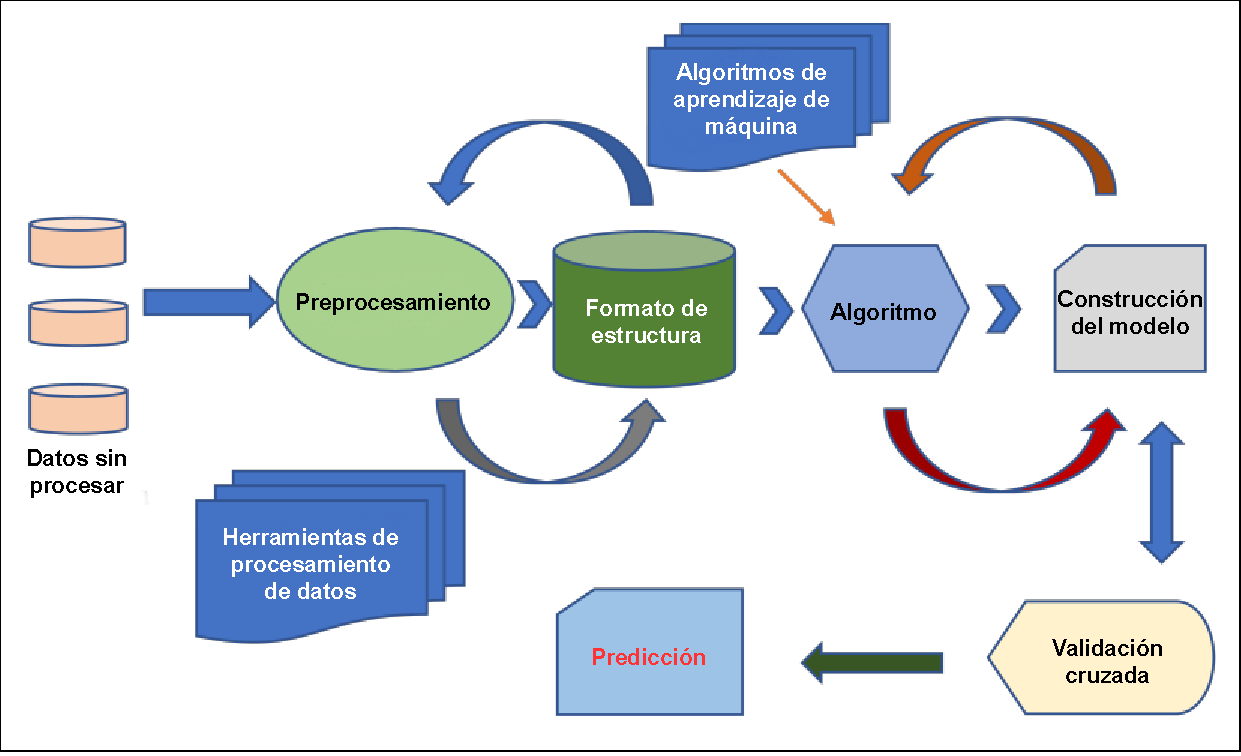
\includegraphics[width=0.8\textwidth]{E_IMAGENES/1_Capitulo2/1-research-background/Paper_1_1.pdf}
  \caption*{Fuente: \citet{9276955}}
  \label{fig:Imagen_1}
\end{figure}

\lipsum[2]

\begin{table}[H]
  \centering
  \caption{Resultados del artículo 1}
  \begin{tabular}{cccc} 
  \hline
  \textbf{Modelo}          & \textbf{Exactitud} & \textbf{Precisión} & \textbf{Sensibilidad}  \\ 
  \hline
  Árbol de
    decisión      & 0.96               & 0.75               & 0.7                    \\ 
  \hline
  Bosque
    aleatorio       & 0.95               & 1                  & 0.17                   \\ 
  \hline
  Naive Bayes
    Gaussiano  & 0.99               & 1                  & 0.88                   \\ 
  \hline
  K vecinos más
    cercanos & 0.93               & 0.44               & 0.23                   \\
  \hline
  \end{tabular}
  \caption*{Fuente: \citet{9276955}}
  \label{tab:Paper_1_3}
\end{table}

\subsubsection{Antecedente 2}

\lipsum[2]

\begin{figure}[H]
  \centering
  \caption{Resultados del enfoque global del artículo 2}
  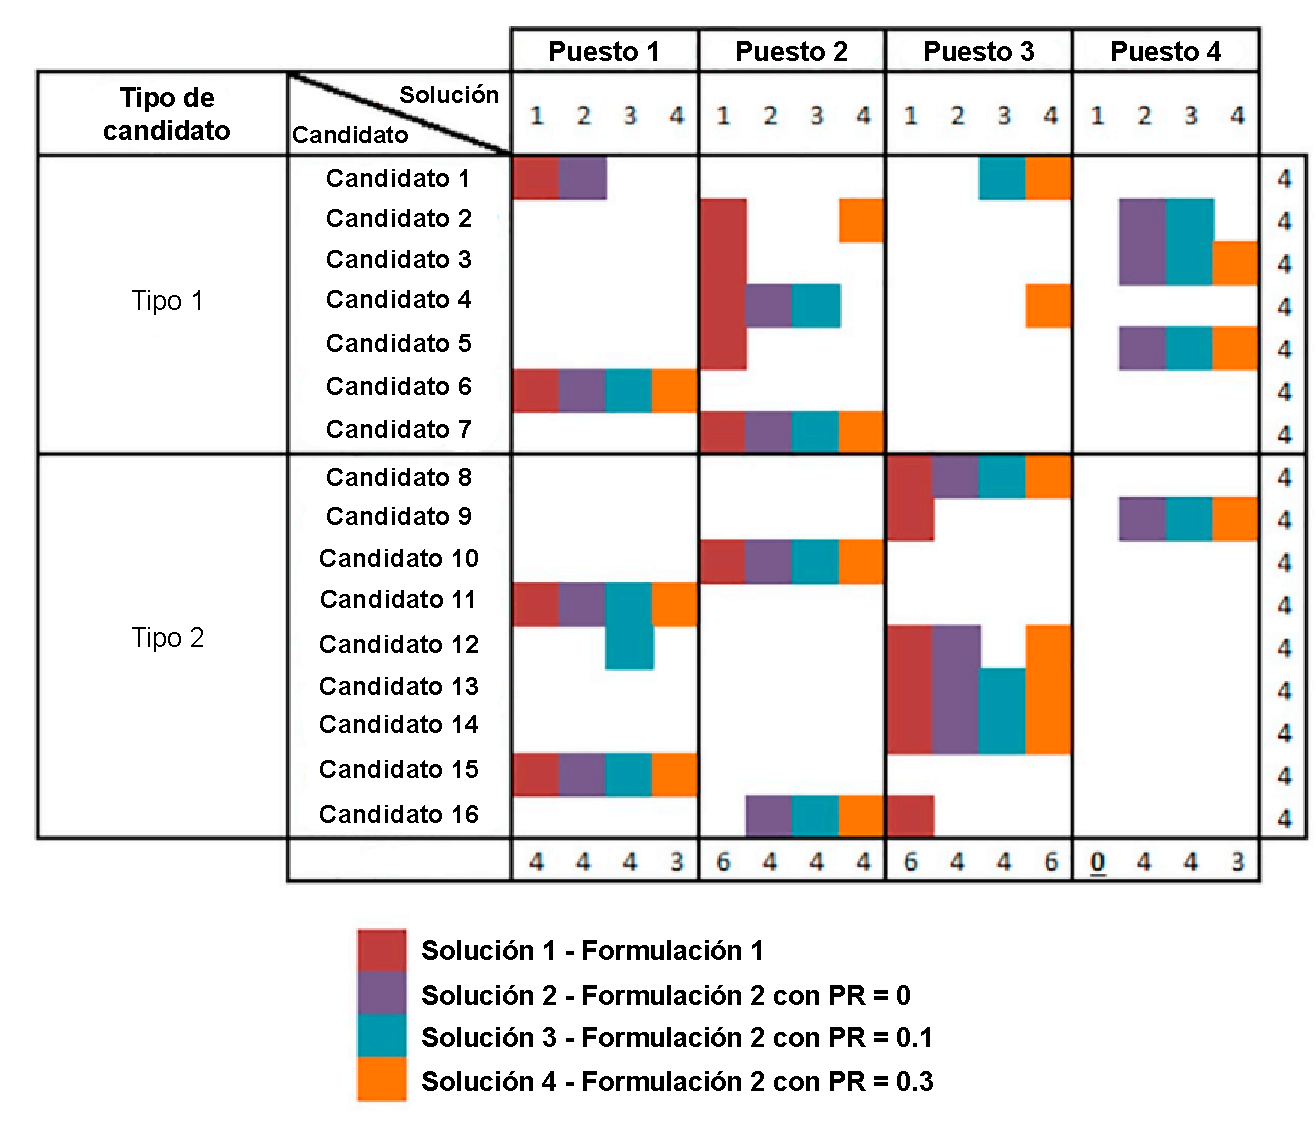
\includegraphics[width=1.0\textwidth]{E_IMAGENES/1_Capitulo2/1-research-background/Paper_2_2.pdf}
  \caption*{Fuente: \citet{PESSACH2020113290}}
  \label{fig:Paper_2_2}
\end{figure}

\subsubsection{Antecedente 3}

\lipsum[3]

\begin{table}[H]
  \centering
  \caption{Resultados del artículo 3}
  \resizebox{\columnwidth}{!}{
    \begin{tabular}{ccccc} 
    \hline
    \begin{tabular}[c]{@{}c@{}}\textbf{Tamaño de la muestra}\end{tabular} & \begin{tabular}[c]{@{}c@{}}\textbf{Exactitud (\%)}\end{tabular} & \begin{tabular}[c]{@{}c@{}}\textbf{Especificidad (\%)}\end{tabular} & \begin{tabular}[c]{@{}c@{}}\textbf{Sensibilidad (\%)}\end{tabular} & \begin{tabular}[c]{@{}c@{}}\textbf{Robustez (\%)}\end{tabular}  \\ 
    \hline
    100                                                                              & 96.2                    & 94.2                        & 94.8                       & 94.5                    \\ 
    \hline
    200                                                                              & 95.4                    & 95.6                        & 95.2                       & 95.4                    \\ 
    \hline
    300                                                                              & 94.8                    & 93.6                        & 93.9                       & 93.7                    \\ 
    \hline
    400                                                                              & 95.8                    & 93.8                        & 95.1                       & 94.6                    \\ 
    \hline
    500                                                                              & 93.2                    & 95.2                        & 92.9                       & 94.3                    \\ 
    \hline
    600                                                                              & 86.2                    & 85.6                        & 86.6                       & 86.2                    \\ 
    \hline
    700                                                                              & 92.8                    & 94.4                        & 94.6                       & 94.5                    \\ 
    \hline
    800                                                                              & 94.4                    & 95.2                        & 94.8                       & 95.1                    \\ 
    \hline
    900                                                                              & 93.8                    & 94.6                        & 95.1                       & 94.8                    \\ 
    \hline
    1000                                                                             & 88.5                    & 87.8                        & 85.6                       & 86.3                    \\ 
    \hline
    1100                                                                             & 94.7                    & 96.2                        & 93.8                       & 94.2                    \\ 
    \hline
    1200                                                                             & 96.1                    & 95.2                        & 93.2                       & 94.5                    \\ 
    \hline
    \textbf{1300}                                                                             & \textbf{96.96}                   & \textbf{96.38}                       & \textbf{96.02}                      & \textbf{96.26}                   \\
    \hline
    \end{tabular}
  }
  \caption*{Fuente: \citet{StackedKNN}}
  \label{tab:Paper_3_4}
\end{table}

\subsubsection{Antecedente 4}

\lipsum[4]

\begin{figure}[H]
  \centering
  \caption{Metodología a usar del artículo 4}
  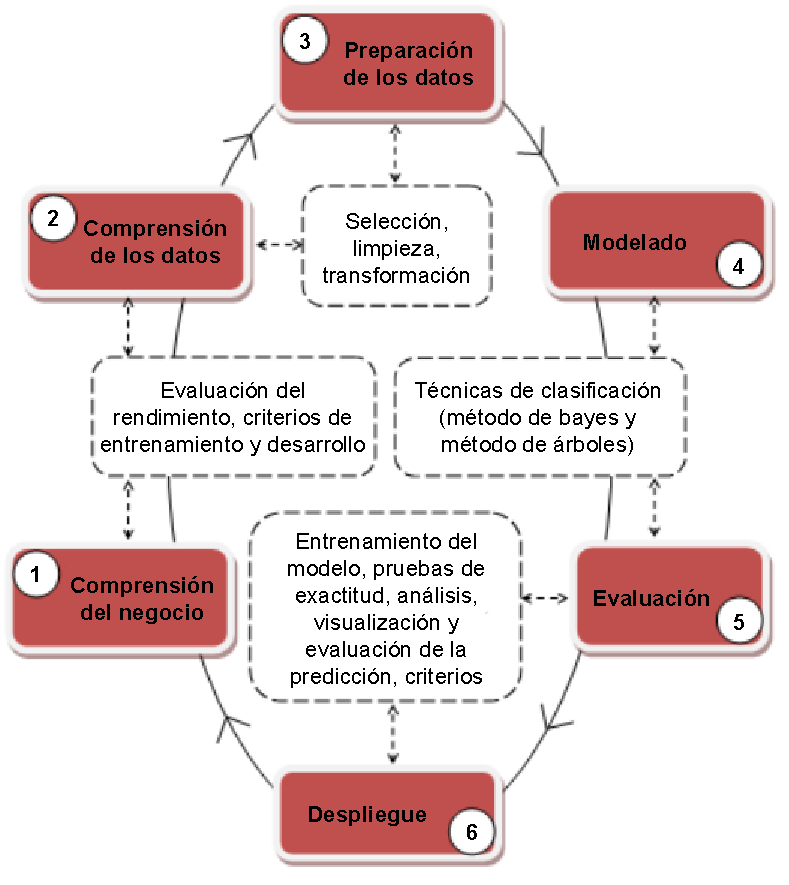
\includegraphics[width=0.8\textwidth]{E_IMAGENES/1_Capitulo2/1-research-background/Paper_4_1.pdf}
  \caption*{Fuente: \citet{arxiv2013}}
  \label{fig:Paper_4_1}
\end{figure}

\subsubsection{Antecedente 5}

\citet{IJET11738} sostiene que, por un lado, los estudiantes deben prepararse desde etapas tempranas de su formación para adaptarse a la vida laboral y evaluar constantemente su desempeño.

Y, por otro lado, los reclutadores primero evalúan a los candidatos en diferentes parámetros y luego eligen en que puesto de trabajo deben mantener al candidato según su desempeño, y en base al aporte que puede realizar a la organización \citep{IJET11738}.

\subsection{Evaluación comparativa}

\lipsum[6]

\subsection{Usos alternativos o aplicaciones varias}

\lipsum[7]

\subsection{Software o sistemas existentes}

\lipsum[8]

\section{BASES TEÓRICAS}

\subsection{Variable dependiente: Nombre de la VD}

\lipsum[9]

\subsection{Variable independiente: Nombre de la VI}

\lipsum[10]

		
	% ESTADO DEL ARTE
	\chapter{MÉTODO DE LA INVESTIGACIÓN}
\markboth{CAPÍTULO \thechapter: MÉTODO DE LA INVESTIGACIÓN}{}
\section{TIPO, NIVEL Y DISEÑO DE LA INVESTIGACIÓN}
\subsection{Tipo de la investigación}

\lipsum[1]

\subsection{Nivel de la investigación}

\lipsum[2]

\subsection{Diseño de la investigación}

\lipsum[3]

\section{VARIABLES Y OPERACIONALIZACIÓN}
\subsection{Variables}
\textbf{Variable independiente:}
Nombre de la VD.

\textbf{Variable dependiente:}
Nombre de la VI.

\subsection{Operacionalización de variables}

\lipsum[2]

\section{POBLACIÓN Y MUESTRA}

\subsection{Población}

\lipsum[3]

\subsection{Muestra}

\lipsum[4]

\section{TÉCNICAS E INSTRUMENTOS DE RECOLECCIÓN DE DATOS, VALIDEZ Y CONFIABILIDAD}

\subsection{Técnicas}

\lipsum[5]

\subsection{Herramientas}

\lipsum[6]

\section{MÉTODOS DE ANÁLISIS DE DATOS}

\lipsum[7]

\subsection{Prueba de hipótesis}

\lipsum[8]

\subsubsection{Prueba de Wilcoxon}

\lipsum[9]

\paragraph{Hipótesis estadísticas}

\lipsum[10]

\section{ASPECTOS LEGALES Y ÉTICOS}

\lipsum[11]

		
	% CAPÍTULO 4
	\chapter{DESARROLLO DE LA SOLUCIÓN}
\markboth{CAPÍTULO \thechapter: DESARROLLO DE LA SOLUCIÓN}{}


\section{METODOLOGÍA DE DESARROLLO DE LA SOLUCIÓN}

\lipsum[1]

\subsection{Paso 1}

\lipsum[2]

\subsection{Paso 2}

\lipsum[3]

\subsection{Paso 3}

\lipsum[4]


\section{APLICACIÓN DE LA METODOLOGÍA}

\lipsum[5]

\subsection{Paso 1}

\lipsum[6]

\subsection{Paso 2}

\lipsum[7]

\subsection{Paso 3}

\lipsum[8]

	% CAPÍTULO 5
	\chapter{RESULTADOS}
\markboth{CAPÍTULO \thechapter: RESULTADOS}{}


\section{RESULTADOS DESCRIPTIVOS}

\lipsum[1]

\subsection{Medidas descriptivas}

\lipsum[2]


\section{RESULTADOS INFERENCIALES}

\lipsum[3]

\subsection{Prueba de normalidad}

\lipsum[4]

\subsection{Prueba de hipótesis}

\lipsum[5]


	% CAPÍTULO 6
	\chapter{DISCUSIÓN DE LOS RESULTADOS}
\markboth{CAPÍTULO \thechapter: DISCUSIÓN DE LOS RESULTADOS}{}
\section{CONTRASTACIÓN DE LA HIPÓTESIS}

\lipsum[1]

\section{CONTRASTACIÓN DE LA HIPÓTESIS CON RESULTADOS SIMILARES}

\lipsum[2]

	
	%Parte FINAL DE LA TESIS
	\backmatter

	% CONCLUSIONES
	\cleardoublepage\phantomsection\addcontentsline{toc}{chapter}{CONCLUSIONES}
\chapter*{CONCLUSIONES}
\markboth{CONCLUSIONES}{}
%--
\begin{enumerate}

    \item Conclusión 1

    \item Conclusión 2

    \item Conclusión 3

\end{enumerate}

	
	% RECOMENDACIONES	
	\cleardoublepage\phantomsection\addcontentsline{toc}{chapter}{RECOMENDACIONES}
\chapter*{RECOMENDACIONES}
\markboth{RECOMENDACIONES}{}
%
\begin{enumerate}

    \item Recomendación 1

    \item Recomendación 2

    \item Recomendación 3

\end{enumerate}
	
	% REFERENCIAS BIBLIOGRÁFICAS
	\cleardoublepage\phantomsection\addcontentsline{toc}{chapter}{REFERENCIAS BIBLIOGRÁFICAS}
\begingroup
\titleformat*{\chapter}{\vspace{4cm}\normalfont\fontsize{14pt}{0}\selectfont\bfseries\centering}
\bibliography{3_3_BIBLIOGRAFIA/library}
\endgroup

	
	% ANEXOS	
	\cleardoublepage\phantomsection\addcontentsline{toc}{chapter}{ANEXOS}
% Cambiar la fuente a 14 temporalmente, y luego regresarla a 11
\begin{center}
    \fontsize{14pt}{0}\selectfont\bfseries{ANEXOS}
    \fontsize{11pt}{11pt}\selectfont
    \markboth{ANEXOS}{}
\end{center}

%---

% Definir númeración y citación para Listing 

%\renewcommand{\lstlistingname}{ Código A \hspace{-1.75mm}}% Cambiar el nombre a Algoritmo
%\renewcommand*{\thelstlisting}{.\arabic{lstlisting}} 
%\def\lstlistingautorefname{Código A\hspace{-0.75mm}}

% Redefinir númeración y citación para Figuras
\renewcommand\thefigure{.\arabic{figure}}
\setcounter{figure}{0}
\renewcommand\figurename{Figura A \hspace{-1.6mm}}
\def\figureautorefname{Figura A \hspace{-2mm}}

\section*{ANEXO A: Matriz de consistencia}
\phantomsection
\addcontentsline{toc}{section}{ANEXO A: Matriz de consistencia}

\begin{figure}[H]
    \begin{adjustbox}{
        addcode={\begin{minipage}{\width}
                     \caption[]{Matriz de consistencia}\label{fig:Anexo_A}}
            {\captionsetup{font=footnotesize,font=bf}
        \caption*{Fuente: La empresa\\Elaboración: Propia}
    \end{minipage}},
rotate=90, center}
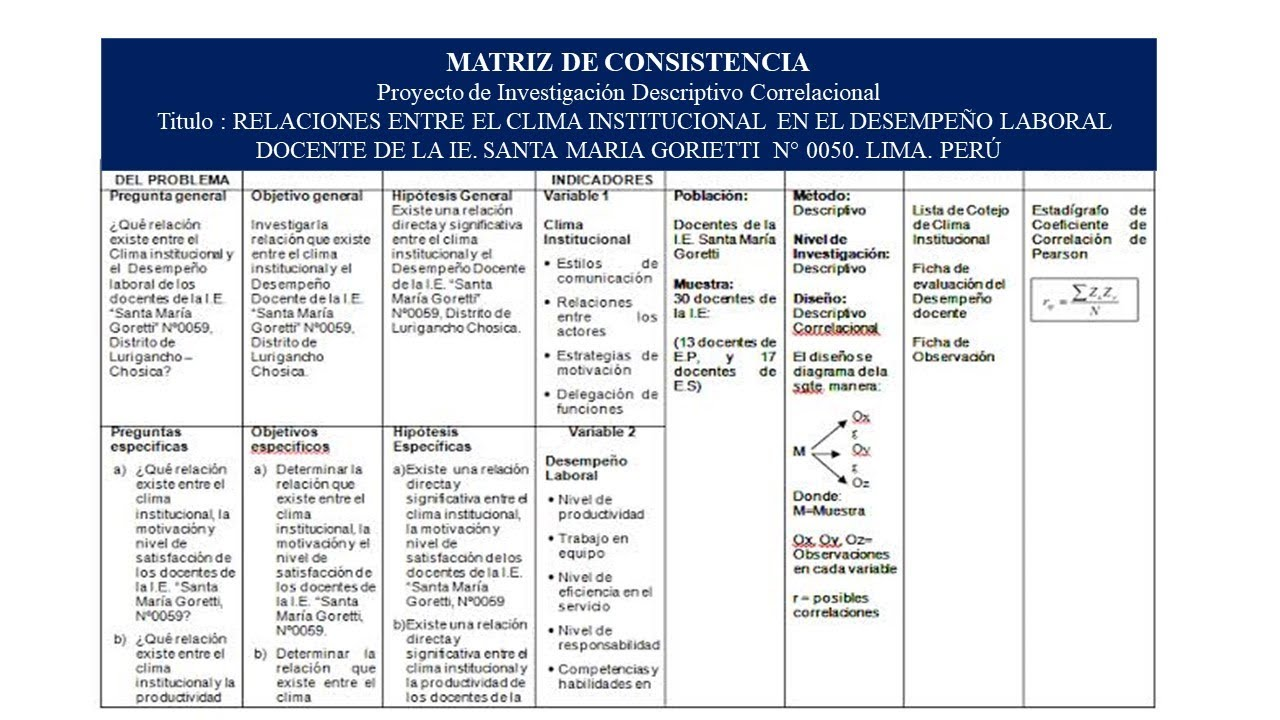
\includegraphics[width=1.2\linewidth]{E_IMAGENES/Anexos/Matriz_consistencia.jpg}
\end{adjustbox}
\end{figure}
\newpage

\section*{ANEXO B: Cronograma}
\phantomsection
\addcontentsline{toc}{section}{ANEXO B: Cronograma}

\begin{figure}[H]
\begin{adjustbox}{
addcode={\begin{minipage}{\width}
\caption[]{Cronograma}\label{fig:Anexo_B}}
{\captionsetup{font=footnotesize,font=bf}
\caption*{Fuente: La empresa\\Elaboración: Propia}
\end{minipage}},
rotate=90, center}
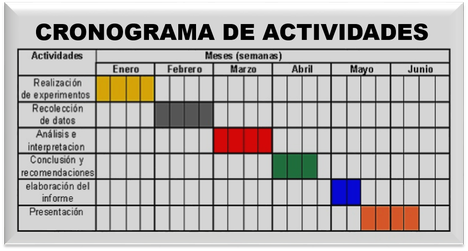
\includegraphics[width=1.0\linewidth]{E_IMAGENES/Anexos/Cronograma.png}
\end{adjustbox}
\end{figure}
\newpage

\section*{ANEXO C: Constancia emitida por la empresa}
\phantomsection
\addcontentsline{toc}{section}{ANEXO C: Constancia emitida por la empresa}

\begin{figure}[H]
\centering
\caption[]{Constancia emitida por la empresa}
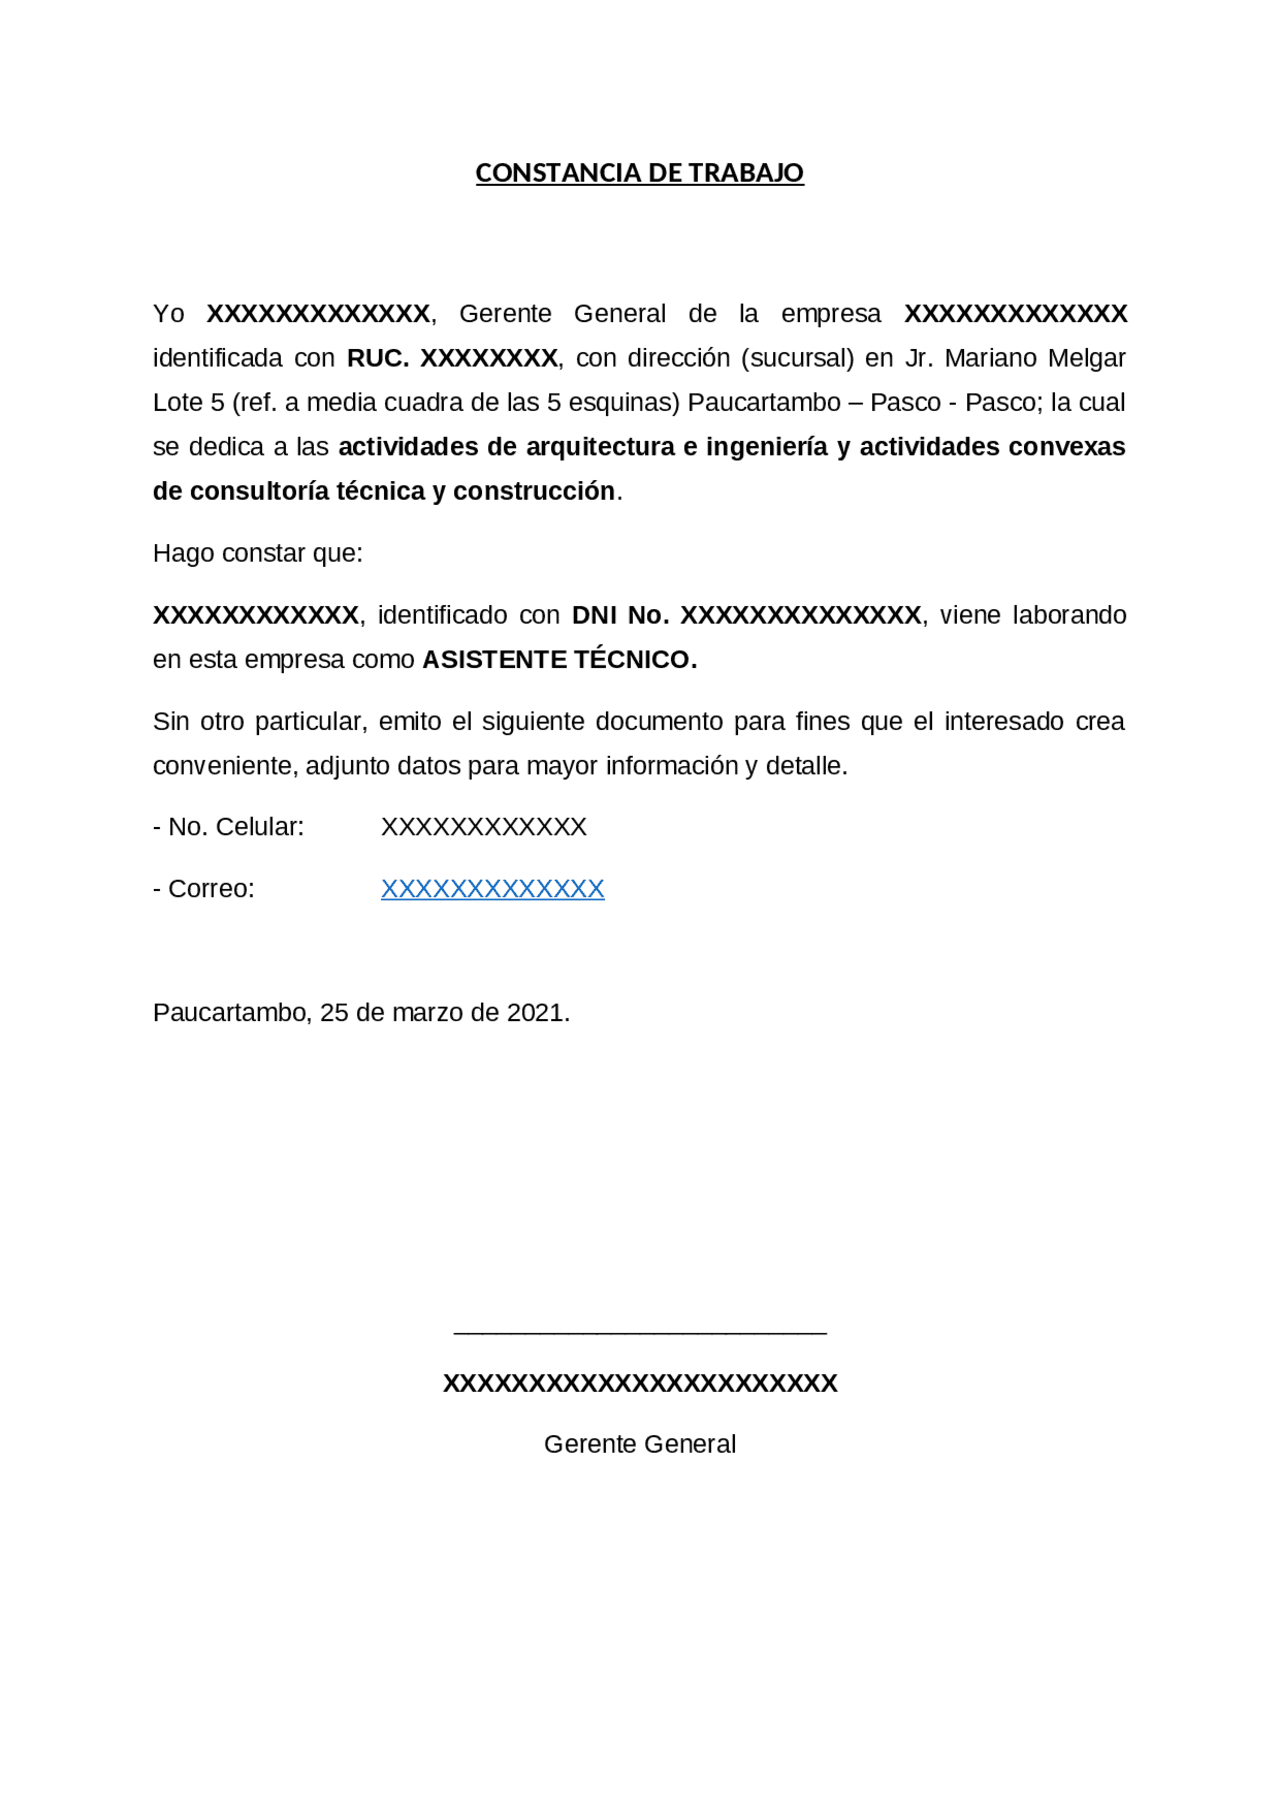
\includegraphics[width=1\linewidth]{E_IMAGENES/Anexos/Constancia_investigacion.png}
\caption*{Fuente: La empresa}
\label{fig:Anexo_C}
\end{figure}

	
\end{document}